%Master File:lectures.tex

\lesson{Eigensystems}
\vspace{-2cm}
\begin{center}
  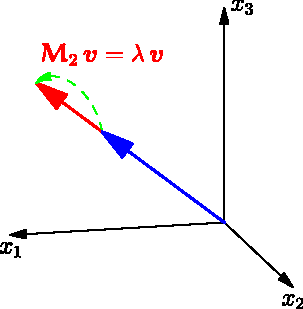
\includegraphics[width=0.4\linewidth]{eigenvector-2}
\end{center}
\keywords{Eigenvectors, Orthogonal Matrices, Eigenvector
  Decomposition, Rank}
%%%%%%%%%%%%%%%%%%%%%%% Next Slide %%%%%%%%%%%%%%%%%%%%%%%
\renewcommand{\Outline}{%
\begin{slide}
\section[1]{Outline}

\begin{minipage}{12cm}
  \begin{enumerate}\squeeze
    \outlineitem{Eigenvectors}{eigenvectors}
    \outlineitem{Orthogonal Matrices}{orthogonal}
    \outlineitem{Eigen Decomposition}{decomposition}
    \outlineitem{Low Rank Approximation}{lowrank}
  \end{enumerate}
\end{minipage}\hfill
\begin{minipage}{10cm}
  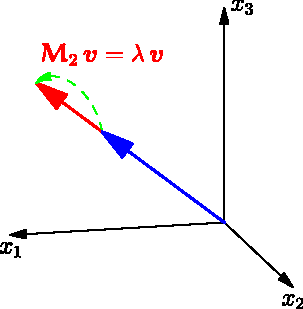
\includegraphics[height=10cm]{eigenvector-2}
\end{minipage}
\end{slide}
\addtocounter{outlineitem}{1}
}

\setcounter{outlineitem}{1}
\Outline % Eigenvectors
\toptarget{firstoutline}

%%%%%%%%%%%%%%%%%%%%%%% Next Slide %%%%%%%%%%%%%%%%%%%%%%%

\begin{slide}
\section[-2]{Eigenvector equation}
\pb

  \begin{itemize}
  \item Eigen-systems help us to understand mappings\pauseh
  \item A vector $\bm{v}$ is said to be an \emph{eigenvector} if
    \begin{minipage}{0.5\linewidth}
      \begin{displaymath}
        \mat{M} \bm{v} = \lambda \, \bm{v}\pauseh
      \end{displaymath}
    \end{minipage}\hfill
    \begin{minipage}{0.4\linewidth}
      \multipdf[height=7cm]{eigenvector}\pause
    \end{minipage}
  \item $\mat{M}$ is square (i.e. $n\stimes n$)\pauseh
  \item Where the number $\lambda$ is the \emph{eigenvalue}\pauseh
  \item Eigenvalues play a fundamental role in understanding operators\pauseh
  \end{itemize}


\end{slide}


%%%%%%%%%%%%%%%%%%%%%%% Next Slide %%%%%%%%%%%%%%%%%%%%%%%

\begin{slide}
\section[-1]{Symmetric Matrices}

\begin{PauseHighLight}
  \begin{itemize}
  \item If $\mat{M}$ is an $n\stimes n$ \emph{symmetric} matrix then it has
    $n$ real orthogonal eigenvectors with real eigenvalues\pause
  \item We denote the $i^{th}$ eigenvector by $\bm{v}_i$ and the
    corresponding eigenvalue by $\lambda_i$ so that
    \begin{displaymath}
      \mat{M} \bm{v}_i = \lambda_i \, \bm{v}_i \pause
    \end{displaymath}
  \item Orthogonal means that if $i\neq j$ then
    \begin{displaymath}
      \bm{v}_i^\tr \, \bm{v}_j = 0\pause
  \end{displaymath}
  \item (We can always normalise eigenvectors if we want)\pause
  \end{itemize}
\end{PauseHighLight}

\end{slide}


%%%%%%%%%%%%%%%%%%%%%%% Next Slide %%%%%%%%%%%%%%%%%%%%%%%

\begin{slide}
\section[-2]{Proof of Orthogonality}

\begin{PauseHighLight}
  \begin{itemize}
  \item $\left(\strut \mat{M}\bm{v}_i = \lambda_i\bm{v}_i\right)^\tr$
    implies $\bm{v}_i^\tr \mat{M}^\tr = \lambda_i\bm{v}_i^\tr$\pause
  \item When $\mat{M}$ is symmetric then $\mat{M}\bm{v}_i = \lambda_i\bm{v}_i
    \Rightarrow \bm{v}_i^\tr \mat{M} = \lambda_i\bm{v}_i^\tr$\pause
  \item Consider two eigenvectors $\bm{v}_i$ and $\bm{v}_j$ of $\mat{M}$
    \begin{align*}
      \bm{v}_i^\tr \mat{M} \bm{v}_j &= (\bm{v}_i^\tr \mat{M}) \bm{v}_j =
      \lambda_i  \bm{v}_i^\tr \bm{v}_j \\
      &= \bm{v}_i^\tr (\mat{M} \bm{v}_j)
      = \lambda_j  \bm{v}_i^\tr \bm{v}_j\pause
    \end{align*}
  \item So either $\lambda_i = \lambda_j$ or $\bm{v}_i^\tr \bm{v}_j=0$\pause
  \item If $\lambda_i = \lambda_j$ then any linear combination of
    $\bm{v}_i$ and $\bm{v}_j$ is an eigenvector
    ($\mat{M} (a\,\bm{v}_i + b\,\bm{v}_j) = \lambda_i (a\,\bm{v}_i +
    b\,\bm{v}_j) $)\pause.  So I can choose two eigenvectors that are
    orthogonal to each other.\pauseb
  \end{itemize}
\end{PauseHighLight}

\end{slide}

%%%%%%%%%%%%%%%%%%%%%%% Next Slide %%%%%%%%%%%%%%%%%%%%%%%
\Outline % Orthogonal Matrices
%%%%%%%%%%%%%%%%%%%%%%% Next Slide %%%%%%%%%%%%%%%%%%%%%%%

\begin{slide}
\section[-2]{Orthogonal Matrices}

\begin{PauseHighLight}
  \begin{itemize}
  \item We can construct an \emph{orthogonal} matrix $\mat{V}$ from the
    eigenvectors
    \begin{displaymath}
      \mat{V} = (\bm{v}_1, \bm{v}_2 , \cdots, \bm{v}_n)\pause
    \end{displaymath}
    \vspace*{-1cm}
  \item Matrix $\mat{V}$ is an $n\stimes n$ matrix\pause
  \item Because of the orthogonality of the vectors $\bm{v}_i$
    \begin{displaymath}
      \mat{V}^\tr \, \mat{V} \pause =
      \begin{pmatrix}
        \bm{v}^\tr_1 \bm{v}_1 & \bm{v}^\tr_1 \bm{v}_2 & \cdots &
        \bm{v}^\tr_1 \bm{v}_n
        \\
        \bm{v}^\tr_2 \bm{v}_1 & \bm{v}^\tr_2 \bm{v}_2 & \cdots &
        \bm{v}^\tr_2 \bm{v}_n
        \\
        \vdots & \vdots & \ddots & \vdots
        \\
        \bm{v}^\tr_n \bm{v}_1 & \bm{v}^\tr_n \bm{v}_2 & \cdots &
        \bm{v}^\tr_n \bm{v}_n
      \end{pmatrix} \pause =
      \begin{pmatrix}
        1 & 0 & \cdots & 0 \\
        0 & 1 & \cdots & 0 \\
        \vdots & \vdots & \ddots & \vdots \\
        0 & 0 & \cdots & 1
      \end{pmatrix} \pause
      = \mat{I}\pause
    \end{displaymath}
  \end{itemize}
\end{PauseHighLight}

\end{slide}

%%%%%%%%%%%%%%%%%%%%%%% Next Slide %%%%%%%%%%%%%%%%%%%%%%%

\begin{slide}
\section[-2]{The Other Way Around}

\begin{PauseHighLight}
  \begin{itemize}
  \item We have shown that $\mat{V}^\tr \, \mat{V} = \mat{I}$\pause
  \item Thus multiply both sides on the left by $\mat{V}$
    \begin{align*}
      \mat{V}\,\mat{V}^\tr \, \mat{V} = \mat{V}\pause
    \end{align*}
  \item $\mat{V}$ will have an inverse,
    $\mat{V}^{-1}$, such that
    $\mat{V} \, \mat{V}^{-1} = \mat{I}$\pause
  \item Multiplying the equation on the right by $\mat{V}^{-1}$
    \begin{align*}
      (\mat{V}\,\mat{V}^\tr) \, \mat{V} \, \mat{V}^{-1}
      &= \mat{V}\,\mat{V}^{-1}\pause  \\
      \mat{V}\,\mat{V}^\tr &= \mat{I}\pauseb
    \end{align*}
  \item Note that, $\mat{V}^{-1}=\mat{V}^\tr$ (definition of
    orthogonal matrix)\pause
  \end{itemize}
\end{PauseHighLight}

\end{slide}

%%%%%%%%%%%%%%%%%%%%%%% Next Slide %%%%%%%%%%%%%%%%%%%%%%%

\begin{slide}
\section[-2]{Invertible Matrices}

\begin{PauseHighLight}
  \begin{itemize}
  \item A matrix, $\mat{M}$, will be singular (uninvertible) if there
    exists a vector $\bm{x}$ ($\neq\bm{0}$) such that
    \begin{align*}
      \mat{M}\,\bm{x} = \bm{0}\pause
    \end{align*}
  \item Now if there exists such a vector such that $\mat{V}\,\bm{x} =
    \bm{0}$ then multiply by $\mat{V}^\tr$ we get
    \begin{align*}
      \mat{V}^\tr\, \mat{V}\, \bm{x} &= \mat{V}^\tr\, \bm{0} \pause \\
      \bm{x} &= \bm{0}
    \end{align*}
    since $\mat{V}^\tr\, \mat{V} = \mat{I}$\pauseb
  \item Thus $\bm{V}$ is invertible\pauseb
  \end{itemize}
\end{PauseHighLight}

\end{slide}



%%%%%%%%%%%%%%%%%%%%%%% Next Slide %%%%%%%%%%%%%%%%%%%%%%%

\begin{slide}
\section[-2]{Rotations}

\begin{PauseHighLight}
  \begin{itemize}
  \item Orthogonal matrices satisfy $\mat{V}^\tr \mat{V} = \mat{V}\,
    \mat{V}^\tr=\mat{I}$\pause
  \item As a consequent they define rotations (and possibly a reflection)\pause
  \item Consider a vector $\bm{x}$ and $\bm{x}'=\mat{V}\bm{x}$, now
    \begin{align*}
      \| \bm{x}' \|_2^2 = \bm{x}^{\prime\tr}\bm{x}'\pause
      = (\mat{V}\bm{x})^\tr (\mat{V}\bm{x})\pause
      = \bm{x}^\tr \mat{V}^\tr \mat{V} \bm{x}\pause
      = \bm{x}^\tr \bm{x} \pause = \| \bm{x} \|_2^2 \pause
    \end{align*}
  \item Similarly if additionally $\bm{y}'=\mat{V}\bm{y}$ then
    {\small
    \begin{align*}
      \langle \bm{x}', \bm{y}' \rangle = (\mat{V}\bm{x})^\tr
      (\mat{V}\bm{y})\pause
       = \bm{x}^\tr \mat{V}^\tr \mat{V} \bm{y}\pause
       = \bm{x}^\tr \bm{y} \pause = \langle \bm{x}, \bm{y} \rangle\pause
       = \| \bm{x} \|_2 \, \| \bm{y} \|_2 \, \cos(\theta)\pause
    \end{align*}}
  \item Rotations and reflections preserve lengths and angles\pause
  \end{itemize}
\end{PauseHighLight}

\end{slide}

%%%%%%%%%%%%%%%%%%%%%%% Next Slide %%%%%%%%%%%%%%%%%%%%%%%
\Outline % Matrix Decompostion
%%%%%%%%%%%%%%%%%%%%%%% Next Slide %%%%%%%%%%%%%%%%%%%%%%%

\begin{slide}
\section[-2]{Matrix Decomposition}

\begin{PauseHighLight}
  \begin{itemize}
  \item Taking the matrix of eigenvectors, $\bm{V}$, then
    \begin{align*}
      \mat{M}\, \mat{V}  &= \mat{M} (\bm{v_1},\bm{v}_2,\ldots,\bm{v}_n)\pause
      =
      (\lambda_1\,\bm{v_1},\lambda_2\,\bm{v}_2,\ldots,\lambda_n\,\bm{v}_n)\pause
      = \mat{V} \,\mat{\Lambda}
    \end{align*}
  \item where $\mat{\Lambda} = \mathrm{diag}(\lambda_1,
    \lambda_2,\ldots, \lambda_n) =
    \begin{pmatrix}
      \lambda_1 & 0 & \cdots & 0 \\
      0 & \lambda_2  & \cdots & 0 \\
      \vdots & \vdots &\ddots &\vdots \\
      0 & 0 & \cdots & \lambda_n
    \end{pmatrix}$\pause
  \item Now
    \begin{align*}
      \mat{M} = \mat{M}\, \mat{V} \, \mat{V}^\tr = \mat{V}
      \,\mat{\Lambda} \, \mat{V}^\tr \pause
    \end{align*}
  \item Very important \textit{similarity transform}\pause
  \end{itemize}
\end{PauseHighLight}

\end{slide}


%%%%%%%%%%%%%%%%%%%%%%% Next Slide %%%%%%%%%%%%%%%%%%%%%%%

\begin{slide}
\section[-2]{Mappings by Symmetric Matrices}

\pb \pause\pauselevel{=1}
\begin{center}
  \multipdf[width=\linewidth]{symmatrixPicture}\pause
\end{center}
\end{slide}


%%%%%%%%%%%%%%%%%%%%%%% Next Slide %%%%%%%%%%%%%%%%%%%%%%%

\begin{slide}
\section[-2]{Inverses}

\begin{PauseHighLight}
  \begin{itemize}
  \item For any square matrix
    \begin{align*}
      \mat{M} &=\mat{V}\,\mat{\Lambda}\,\mat{V}^\tr \pause &
      \mat{M}^{-1} &=\mat{V}\,\mat{\Lambda}^{-1}\,\mat{V}^\tr
    \end{align*}
  \item Where $\mat{\Lambda}^{-1} = \diag(\tfrac{1}{\lambda_1},
    \tfrac{1}{\lambda_2}, \ldots, \tfrac{1}{\lambda_n}) =
    \begin{pmatrix}
      \tfrac{1}{\lambda_1} & 0 & \cdots & 0 \\
      0 & \tfrac{1}{\lambda_2}  & \cdots & 0 \\
      \vdots & \vdots &\ddots &\vdots \\
      0 & 0 & \cdots & \tfrac{1}{\lambda_n}
    \end{pmatrix}$\pause
  \item Since
    \begin{align*}
       \mat{M}\,\mat{M}^{-1} &= (\mat{V}\,\mat{\Lambda}\,\mat{V}^\tr)\,
       (\mat{V}\,\mat{\Lambda}^{-1}\,\mat{V}^\tr)\pause
       = \mat{V}\,\mat{\Lambda}\,(\mat{V}^\tr\,
       \mat{V})\,\mat{\Lambda}^{-1}\,\mat{V}^\tr\pause \\
       &= \mat{V}\,\mat{\Lambda}\,\mat{\Lambda}^{-1}\,\mat{V}^\tr\pause
       = \mat{V}\,\mat{V}^\tr = \mat{I}\pause
    \end{align*}
  \item I.e, Small eigenvalues become large eigenvalues and visa verse\pause
  \end{itemize}
\end{PauseHighLight}

\end{slide}

%%%%%%%%%%%%%%%%%%%%%%% Next Slide %%%%%%%%%%%%%%%%%%%%%%%

\begin{slide}
\section[-1.5]{Ill-Conditioning Again}

\pb\pause\pauselevel{=1}
\begin{center}
  \multipdf[width=0.9\linewidth]{conditioning}\pause
\end{center}

\end{slide}

%%%%%%%%%%%%%%%%%%%%%%% Next Slide %%%%%%%%%%%%%%%%%%%%%%%

\begin{slide}
\section[-2]{Condition Number}

\begin{PauseHighLight}
  \begin{itemize}\squeeze
  \item Taking matrix inverses can be inherently unstable\pause
  \item Any small error can be amplified by taking the inverse\pause
  \item The stability of the inverse depends on the ratio of smallest
    eigenvalue to the largest eigenvalue (i.e. the biggest possible
    amplification compared to the smallest)\pause
  \item Note that the Hilbert-norm of a matrix is the absolute value of
    the largest eigenvalue\pause
  \item The condition number is given by
    \begin{align*}
      \|\mat{M}\|_H \times \|\mat{M}^{-1}\|_H =
      \frac{|\lambda_{\text{\small max}}|}{|\lambda_{\text{\small min}}|}\pause
    \end{align*}
  \item Large condition number implies very ill-conditioned\pause
  \end{itemize}
\end{PauseHighLight}

\end{slide}

%%%%%%%%%%%%%%%%%%%%%%% Next Slide %%%%%%%%%%%%%%%%%%%%%%%
\Outline % Low Rank Approximation
%%%%%%%%%%%%%%%%%%%%%%% Next Slide %%%%%%%%%%%%%%%%%%%%%%%

\begin{slide}
\section[-1]{Rank of a Matrix}

\begin{PauseHighLight}
  \begin{itemize}
  \item The rank of a matrix, $\mat{M}$, is the number of non-zero
    eigenvalues\pause
  \item The space spanned by the eigenvectors $\bm{v}_a$, $\bm{v}_b$,
    etc.{} with zero eigenvalue forms a \emph{null space}\pause
  \item Any vector in the null space will get projected to the zero
    vector
    \begin{align*}
      \mat{M} \, (a\, \bm{v}_a + b \, \bm{v}_b + \cdots) = \bm{0}\pause
    \end{align*}
  \item A square matrix is said to be \emph{rank deficient} if it has
    any eigenvectors with eigenvalue equal to 0\pause
   \item This happens when the columns of the matrix are not linearly independent\pause
 \end{itemize}
\end{PauseHighLight}

\end{slide}

%%%%%%%%%%%%%%%%%%%%%%% Next Slide %%%%%%%%%%%%%%%%%%%%%%%

\begin{slide}
\section[-2]{``Inverting'' Rank Deficient Matrices}

\begin{PauseHighLight}
  \begin{itemize}
  \item Rank deficient matrices are non-invertible (i.e. we don't know
    the vector $\bm{x}$ such that $\mat{M} \bm{x} = \bm{b}$) as we don't know
    the component of the $\bm{x}$ in the null space\pause
  \item Although we don't know $\bm{x}$ we can find a vector,
    $\bm{x}$, that satisfies $\mat{M} \bm{x} = \bm{b}$\pause
  \item Given a symmetric $n\times n$ matrix with $k$ non-zero eigenvalues
    $\lambda_1$, $\lambda_2$, $\ldots$, $\lambda_k$ we can construct
    a ``pseudo inverse'' $\mat{M}^{+}$ as $\mat{V} \mat{\Lambda}^+
    \mat{V}^\tr$ where  $\mat{\Lambda}^{+} = \diag(\tfrac{1}{\lambda_1},
    \tfrac{1}{\lambda_2}, \ldots, \tfrac{1}{\lambda_k}, 0, \ldots,0)$\pause
  \item This finds the vector $\bm{x}$ with no component in the null
    space\pause{} (it is the solution with the smallest norm)\pauseb
  \item This is a different to the pseudo inverse for non-square matrices\pause
  \end{itemize}
\end{PauseHighLight}

\end{slide}

%%%%%%%%%%%%%%%%%%%%%%% Next Slide %%%%%%%%%%%%%%%%%%%%%%%

\begin{slide}
\section{Low Rank Approximation}

\begin{PauseHighLight}
  \begin{itemize}
  \item Recall that matrices with large and small eigenvectors are
    ill-conditions so the inverse has the potential to greatly amplify any
    measurement error\pause
  \item One work around is to set all small eigenvalues to zero and
    use the pseudo inverse\pause
  \item Setting small eigenvalues to zero reduces the rank of the
    matrix and is an example of a low rank approximation\pause
  \item Low rank approximations are much used to obtain approximate
    models for arrays of data\pause{} (we will revisit this when we look at SVD)\pauseb
  \end{itemize}
\end{PauseHighLight}

\end{slide}




%%%%%%%%%%%%%%%%%%%%%%% Next Slide %%%%%%%%%%%%%%%%%%%%%%%

\begin{slide}
\section{Summary}

\begin{PauseHighLight}
  \begin{itemize}
  \item Linear mappings are commonly used in machine learning algorithms
    such as regression\pause
  \item We can understand symmetric operators by looking at their eigenvectors\pause
  \item Any symmetric matrix can be decomposed as $\mat{M} = \mat{V}
    \mat{\Lambda} \mat{V}^\tr$
    \begin{itemize}
    \item where $\mat{V}$ are orthogonal matrices whose rows are the eigenvector
    \item and $\mat{\Lambda}$ is a diagonal matrix of the eigenvalues\pause
    \end{itemize}
  \item This decomposition allows us to understand inverse mappings\pause
  \end{itemize}
\end{PauseHighLight}

\end{slide}


%%% Local Variables:
%%% TeX-master: "lectures"
%%% End:
